% ---------------------------------------------------------------------
% 2.10 Métricas de evaluación
% ---------------------------------------------------------------------
\section[MÉTRICAS DE EVALUACIÓN]{Métricas de evaluación}
\label{sec:metricas}

El desempeño de un sistema basado en la P300 puede evaluarse en dos niveles: el de la
clasificación de cada época como objetivo o no objetivo, que mide la calidad del modelo de
aprendizaje profundo, y el del sistema completo, que mide qué tan rápido y con qué exactitud el
usuario logra seleccionar caracteres.

\subsection{Matriz de confusión}

En un problema de clasificación binaria, las predicciones del modelo pueden compararse con las
etiquetas reales mediante una tabla cruzada conocida como matriz de confusión, representada en la
Figura~\ref{fig:confusion}. Sus cuatro celdas son las siguientes
\cite{fawcett2006}:
\begin{itemize}
  \item \textbf{Verdaderos positivos (TP):} épocas con P300 clasificadas correctamente.
  \item \textbf{Falsos positivos (FP):} épocas sin P300 clasificadas como positivas.
  \item \textbf{Verdaderos negativos (TN):} épocas sin P300 clasificadas correctamente.
  \item \textbf{Falsos negativos (FN):} épocas con P300 que el modelo no detectó.
\end{itemize}

\begin{figure}[htbp]
\centering
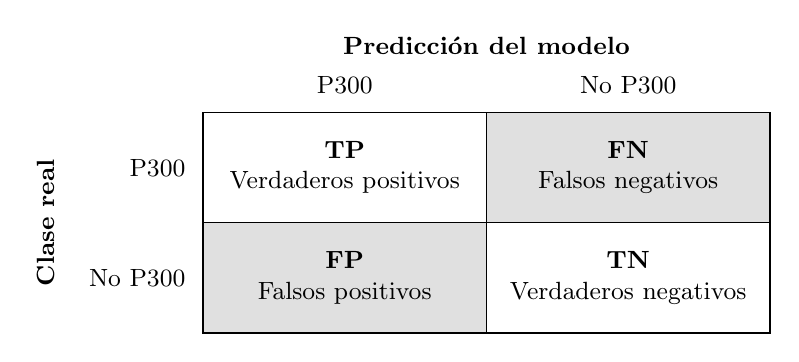
\begin{tikzpicture}[celda/.style={draw, minimum width=3.6cm, minimum height=1.4cm, align=center, font=\small}]
  \node[celda, fill=white] (tp) at (0,0) {\textbf{TP}\\Verdaderos positivos};
  \node[celda, fill=gray!24] (fn) at (3.6,0) {\textbf{FN}\\Falsos negativos};
  \node[celda, fill=gray!24] (fp) at (0,-1.4) {\textbf{FP}\\Falsos positivos};
  \node[celda, fill=white] (tn) at (3.6,-1.4) {\textbf{TN}\\Verdaderos negativos};
  \node[font=\small] at (0,1.05) {P300};
  \node[font=\small] at (3.6,1.05) {No P300};
  \node[font=\small\bfseries] at (1.8,1.55) {Predicción del modelo};
  \node[font=\small, anchor=east] at (-1.9,0) {P300};
  \node[font=\small, anchor=east] at (-1.9,-1.4) {No P300};
  \node[font=\small\bfseries, rotate=90] at (-3.8,-0.7) {Clase real};
\end{tikzpicture}
\caption{Matriz de confusión para la clasificación binaria de épocas. Elaboración propia.}
\label{fig:confusion}
\end{figure}

\subsection{Métricas de clasificación}

A partir de estos cuatro valores se calculan las métricas que se presentan en la
Tabla~\ref{tab:metricas}. La exactitud mide el porcentaje total de aciertos, pero en un conjunto con
una proporción de 1 a 5 entre clases puede engañar, como se vio en la Sección~\ref{sec:speller}.
Por eso se complementa con la sensibilidad, que indica qué proporción de las épocas con P300 fueron
detectadas, con la precisión, que indica qué proporción de las detecciones fueron correctas, y con
el F1-score, que es la media armónica de ambas \cite{fawcett2006}.

\begin{table}[htbp]
\centering
\caption{Métricas de evaluación para la clasificación binaria}
\label{tab:metricas}
\small
\renewcommand{\arraystretch}{1.8}
\begin{tabularx}{\textwidth}{|L{2.8cm}|Y|L{4.4cm}|}
\hline
\textbf{Métrica} & \textbf{Descripción} & \textbf{Fórmula} \\ \hline
Exactitud (\textit{accuracy}) & Proporción de predicciones correctas sobre el total. & $\dfrac{TP+TN}{TP+TN+FP+FN}$ \\[10pt] \hline
Precisión (\textit{precision}) & Proporción de épocas clasificadas como P300 que realmente lo son. & $\dfrac{TP}{TP+FP}$ \\[10pt] \hline
Sensibilidad (\textit{recall}, TPR) & Proporción de épocas con P300 que fueron detectadas. & $\dfrac{TP}{TP+FN}$ \\[10pt] \hline
F1-score & Media armónica entre precisión y sensibilidad. & $2\cdot\dfrac{\text{Precisión}\cdot\text{Sensibilidad}}{\text{Precisión}+\text{Sensibilidad}}$ \\ \hline
\end{tabularx}
\par\smallskip{\footnotesize Elaboración propia con información de \cite{fawcett2006}.}
\end{table}

\subsection{Curva ROC y área bajo la curva}

Los clasificadores de la P300 suelen producir un puntaje continuo, y la etiqueta final depende del
umbral que se elija: al disminuirlo se detectan más épocas con P300, pero también aumentan los
falsos positivos. La curva ROC (\textit{Receiver Operating Characteristic}) representa este
compromiso. Para ello, grafica la sensibilidad contra la proporción de épocas sin P300
clasificadas como positivas en todos los umbrales posibles. El área bajo esta curva (AUC) resume el desempeño en un solo número. Este valor
indica la probabilidad de que el clasificador dé un puntaje mayor a una época positiva que a una
negativa, ambas elegidas al azar \cite{fawcett2006}. Un AUC de 0.5 corresponde a un clasificador
aleatorio, en el que los puntajes de ambas clases se superponen. Un AUC de 1 indica una separación
perfecta. Esta es la métrica utilizada en los trabajos de Alvarado-González et al.
y de Contreras. Este último la considera aceptable a partir de 0.7 \cite{alvarado2021,contreras2021}.

\subsection{Métricas a nivel de sistema}

Una alta AUC en la clasificación de épocas no garantiza por sí sola una comunicación eficiente,
pues la velocidad depende también del número de repeticiones necesarias para seleccionar cada
carácter. En los sistemas de deletreo se reporta además la exactitud por carácter en función
del número de repeticiones, los caracteres por minuto y la tasa de transferencia de información
(ITR), que de acuerdo con Wolpaw et al. se calcula en bits por selección como
\cite{wolpaw2000,wolpaw2002}
\begin{equation}
B = \log_2 N + P\log_2 P + (1-P)\log_2\!\left(\frac{1-P}{N-1}\right),
\label{eq:itr}
\end{equation}
donde $N$ es el número de opciones posibles, 36 en una matriz de $6\times6$, y $P$ es la exactitud
por carácter. Al multiplicar $B$ por el número de selecciones por minuto se obtiene la ITR en bits
por minuto. Con la misma exactitud, usar menos repeticiones sube la ITR porque caben más
selecciones en un minuto. En la práctica, sin embargo, menos repeticiones también bajan la
exactitud, y el número óptimo de repeticiones queda en el punto donde la ganancia en velocidad
todavía compensa los errores.
